Créée en 1964 par Georges Matheron et Jean Serra à l'École des Mines de Paris, la morphologie mathématique est un sous-domaine à la fois théorique et technique des mathématiques et de l'informatique, étroitement lié à l'algèbre, à la théorie des treillis et à la topologie, et qui est en particulier appliqué dans le domaine du traitement d'images \cite{Serra_1983}. Il met en œuvre des techniques de filtrage non linéaire à l'aide de formes géométriques, telles qu'un carré, une croix, un disque, ou toute autre forme encore, appelées << éléments structurants >>, qui sondent le contenu des images et en modifient les propriétés morphologiques \cite{Serra_1986}. \\

\vspace{-2mm}
Les opérations fondamentales de la morphologie mathématique sont l'érosion et la dilatation (fig. \ref{fig:morpho_operations_example}). En les combinant, on peut créer des opérations plus avancées, telles que l'ouverture (érosion puis dilatation) et la fermeture (dilatation puis érosion), ou encore le gradient morphologique (dilatation moins érosion). Ces opérations de morphologie mathématique sont typiquement appliquées dans des contextes où l'élément structurant est binaire, et où l'image elle-même peut être soit binaire, soit en niveaux de gris. Ces opérations peuvent également être généralisées à des fonctions structurantes, c'est-à-dire des éléments structurants en niveaux de gris \cite{Haralick_1987, Serra_1992}. \\

\vspace{-2mm}
\begin{figure}[h]
  \begin{center}

\begin{minipage}{0.49\linewidth}
    \begin{minipage}{0.3\linewidth}
        \centering
        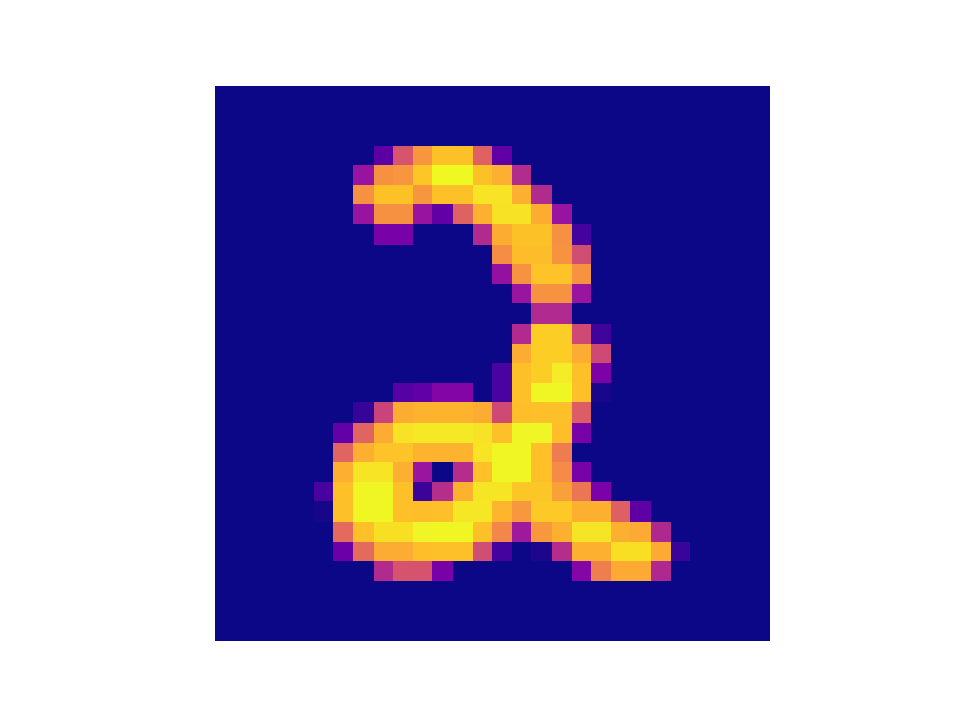
\includegraphics[width=1.0\textwidth]{figures/original.pdf}
    \end{minipage}%
    \begin{minipage}{0.04\linewidth}
        \centering
        \large $\ominus$
    \end{minipage}%
    \begin{minipage}{0.2\linewidth}
        \centering
        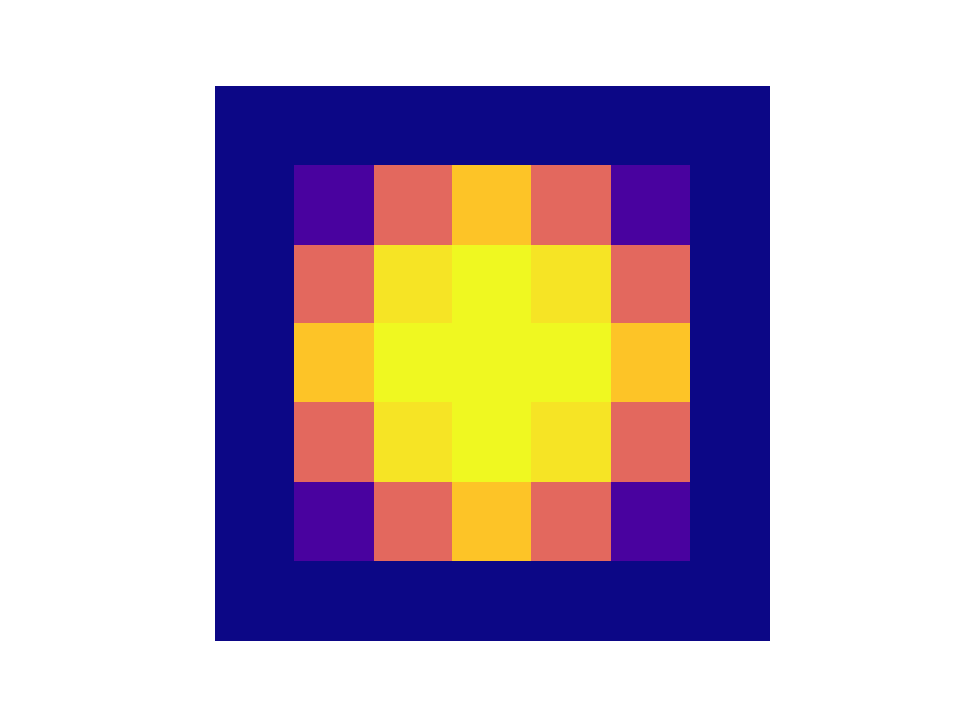
\includegraphics[width=0.7\linewidth]{figures/selem.pdf}
    \end{minipage}% 
    \begin{minipage}{0.06\linewidth}
        \centering
        \large $=$
    \end{minipage}%
    \begin{minipage}{0.3\linewidth}
        \centering
        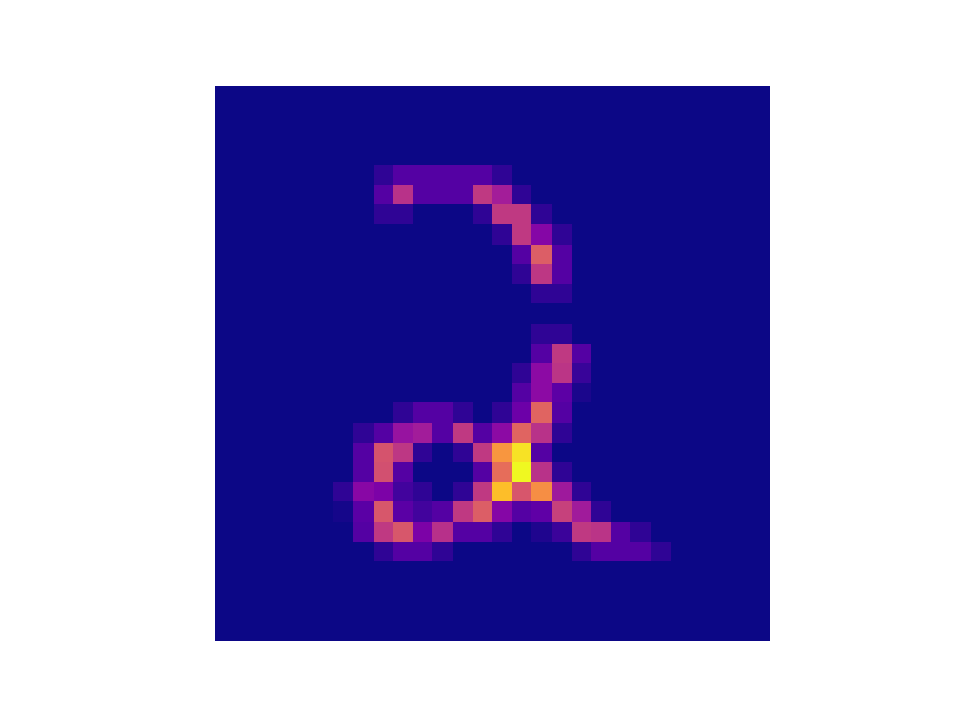
\includegraphics[width=1.0\textwidth]{figures/eroded.pdf}
    \end{minipage}
\end{minipage}%
\hfill%
\begin{minipage}{0.49\linewidth}
    \begin{minipage}{0.3\linewidth}
        \centering
        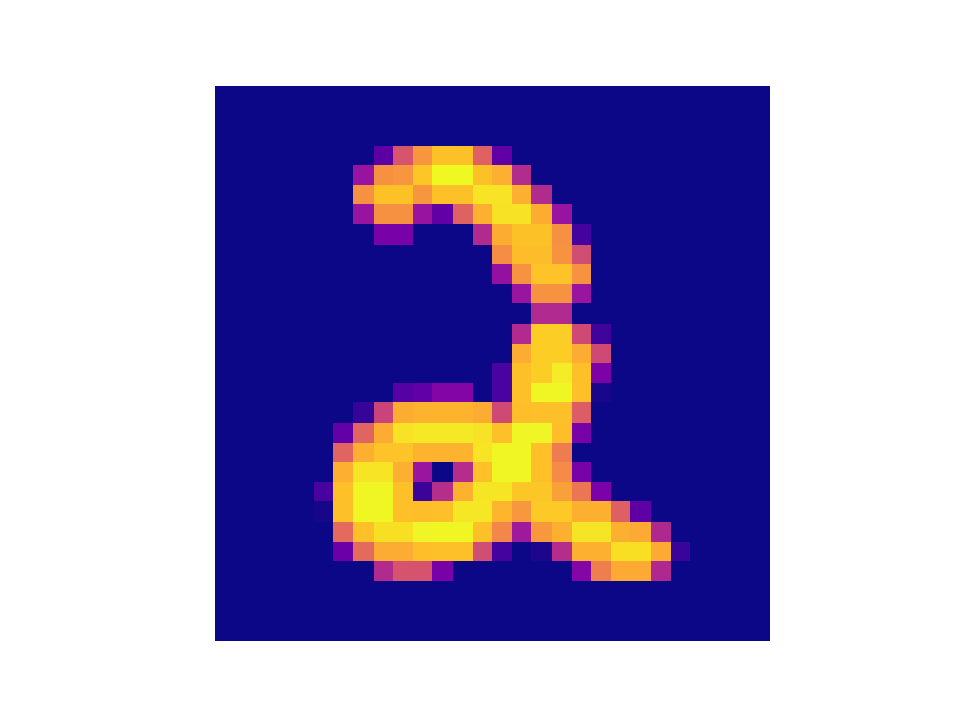
\includegraphics[width=1.0\textwidth]{figures/original.pdf}
    \end{minipage}%
    \begin{minipage}{0.04\linewidth}
        \centering
        \large $\oplus$
    \end{minipage}%
    \begin{minipage}{0.2\linewidth}
        \centering
        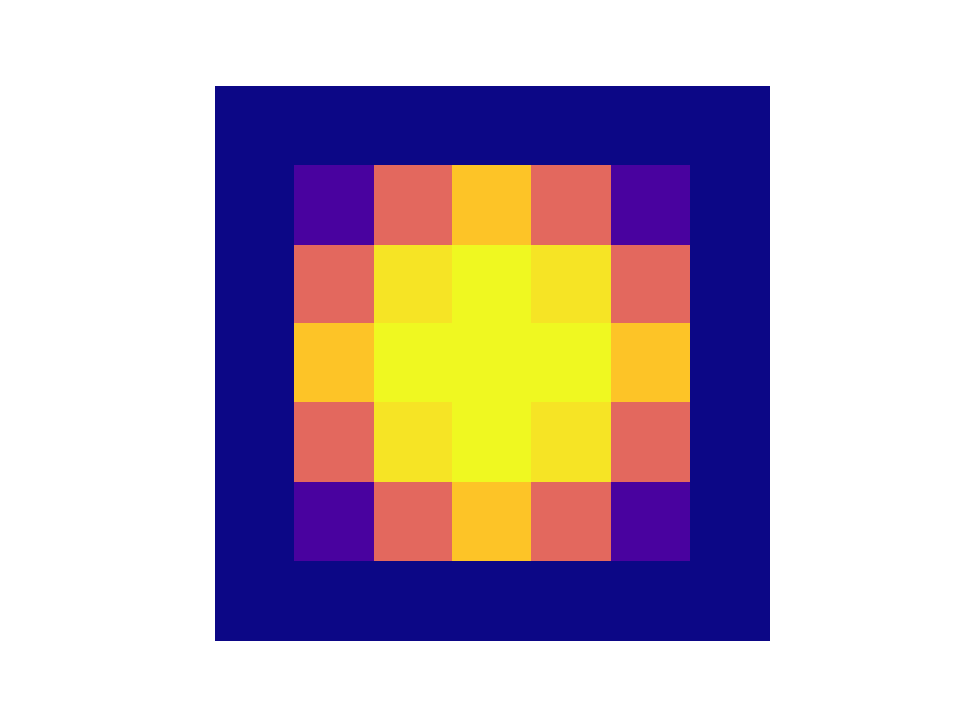
\includegraphics[width=0.7\linewidth]{figures/selem.pdf}
    \end{minipage}% 
    \begin{minipage}{0.06\linewidth}
        \centering
        \large $=$
    \end{minipage}%
    \begin{minipage}{0.3\linewidth}
        \centering
        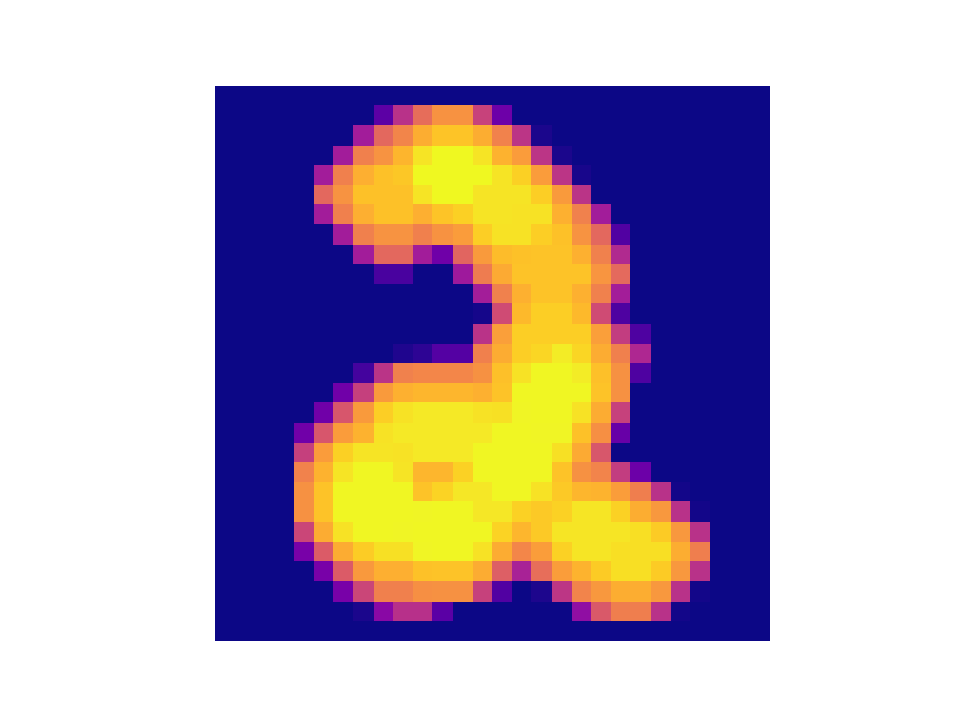
\includegraphics[width=1.0\textwidth]{figures/dilated.pdf}
    \end{minipage}
\end{minipage}%
    
    \caption{\centering Exemple d'une érosion $\ominus$ (à gauche) et d'une dilatation $\oplus$ (à droite) par une fonction structurante $B$ circulaire sur une image en niveaux de gris de la banque MNIST.}
    \label{fig:morpho_operations_example}
  \end{center}
\end{figure}

\vspace{-4mm}
La morphologie mathématique démontre une grande efficacité dans diverses applications de traitement d'images, telles que le débruitage et la détection d'objets \cite{Peters_1995, Horgan_1998}. Cependant, ces performances sont souvent tributaires du niveau d'expertise de l'utilisateur, ainsi que de sa capacité à déterminer la séquence appropriée des opérations fondamentales et à définir adéquatement les éléments structurants associés à la tâche en question. Par conséquent, l'automatisation de la définition des types d'opérations morphologiques et de leurs éléments structurants pour des applications spécifiques représente une perspective particulièrement séduisante. \\

\vspace{-2mm}
Récemment, plusieurs initiatives ont vu le jour en vue d'intégrer l'apprentissage automatique de séquences d'opérations morphologiques au sein des réseaux de neurones convolutionnels \cite{Masci_2012, Hermary_2022, Bloch_2021}. L'objectif est de remplacer les couches de convolution classiques par des couches morphologiques, capables d'apprendre et d'appliquer des érosions ou des dilatations. Les poids des filtres en jeu jouent alors un rôle analogue à celui des fonctions structurantes correspondantes.

%%% NEW PAGE %%%
\newpage

Cependant, en raison du caractère localement non différentiable des opérations morphologiques, qui reposent sur des minimas (érosion) ou maximas (dilatation) ensemblistes, des approches détournées doivent être mises en œuvre pour assurer une convergence optimale du réseau durant la phase d'apprentissage. Deux stratégies ont émergé dans la littérature : l'emploi d'approximations continues et différentiables des opérateurs de minimum et de maximum \cite{Masci_2012, Shih_2019, Kirszenberg_2021, Hermary_2022}, ou le traitement de la couche morphologique de manière similaire à la gestion des opérations localement non différentiables dans les architectures classiques (comme le max-pooling) \cite{Keiller_2019, Roy_2021}. \\

\vspace{-1.6mm}
Dans le cadre de l'emploi d'approximations différentiables du min et du max, la première couche morphologique fonctionnelle, la $p$Conv, a été proposée en 2012 en utilisant la formule de la moyenne contre-harmonique \cite{Masci_2012}. Plus récemment encore, ont été proposées dans \cite{Kirszenberg_2021}, et étendu dans \cite{Hermary_2022}, deux nouvelles couches morphologiques, la $\mathcal{L}$Morph et la $\mathcal{S}$Morph, qui reposent sur d'autres formules d'approximation. Ces couches sont capables d’apprendre de manière très performantes les opérations d’érosion, de dilatation, d'ouverture et de fermeture ainsi que l’élément structurant associé. Cependant, certaines propriétés de ces couches restent mal comprises, voire incomprises, en particulier dans les cas où l’apprentissage est un échec. \\

\vspace{-1.6mm}
L’objectif ici est donc d’explorer plus en profondeur le comportement de ces couches morphologiques différentiables, aussi bien sur des aspects théoriques (comportement asymptotique, morphologie de l'espace de la fonction de perte, convergence durant la phase d’apprentissage, impact de contraintes géométriques, etc.) que pratiques (analyse de la convergence des réseaux, des résultats d'apprentissage sous contrainte, de l'impact d'un partage de poids, etc.). Il s'agira en particulier d'apporter des solutions aux problèmes de convergence des réseaux associés. \\

\vspace{-1.6mm}
Dans leur article, R. Hermary et al. \cite{Hermary_2022} mettent en évidence de meilleures performances de convergence pour les couches $\mathcal{S}$Morph par rapport aux autres couches morphologiques existant. Les études et résultats dont ce rapport fait la synthèses seront ainsi focalisées sur ces couches-ci. Les solutions apportées pour améliorer la convergence des réseaux associés à ces couches, dits $\mathcal{S}$MorphNet, pourront aussi bien toucher la définition même des couches, que la structure des réseaux associés construits, ou que la définition de la fonction de perte lors de la phase d'entraînement. \\

\vspace{-1.6mm}
Dans un premier temps seront passées en revue les différentes méthodes de la littérature : la définition des opérateurs classiques de la morphologie mathématique, la structure des différentes couches morphologiques proposées existant, l'efficacité de convergence des réseaux correspondants vers la structure neuronale cible, ainsi que les différents cas d'échec persistants.
Dans un second temps seront présentées de manière théorique les différentes contributions apportées ainsi que les résultats pratiques de leur application, avant de comparer la convergence des réseaux améliorés à celle des réseaux existant de la littérature dans un dernier temps.
